\documentclass[a4paper,12pt]{amsart}

\usepackage{amsmath}
\usepackage{hyperref}
\usepackage{tikz}
\usepackage{tikz-3dplot}

\title{03 -- The dot product}

\begin{document}
    
    \tdplotsetmaincoords{60}{120}

    \maketitle
    \tableofcontents

    \section{Definition}

    \subsection{Scalar (dot) product}

    The \textbf{scalar} or \textbf{dot product} is a function $\cdot: F^n \times F^n \to F$. It takes two vectors and outputs an element of the field of scalars for the vector space. Given two vectors $\mathbf{u} = (u_1, u_2, \ldots, u_n)$ and $\mathbf{v} = (v_1, v_2, \ldots, v_n)$ it is defined as the sum product 
    \[ \mathbf{u} \cdot \mathbf{v} = \sum_{i=1}^n u_i v_i. \]

    \subsection{Examples}

    Consider the vectors $\mathbf{v}_1 = \begin{pmatrix} 2 \\ 1 \end{pmatrix}$ and $\mathbf{v}_2 = \begin{pmatrix} -3 \\ 5 \end{pmatrix}$. Their dot product is then
    \[ \mathbf{v}_1 \cdot \mathbf{v}_2 = 2 \times (-3) + 1 \times 5 = -6 + 5 = -1. \]

    We have a similar process for three-dimensional real vectors. Let $\mathbf{v}_1 = \begin{pmatrix} 1 \\ 0 \\ -1 \end{pmatrix}$ and $\mathbf{v}_2 = \begin{pmatrix} 1 \\ 0 \\ 1 \end{pmatrix}$. Their dot product is
    \[ \mathbf{v}_1 \cdot \mathbf{v}_2 = 1 \times 1 + 0 \times 0 + 1 \times (-1) = 1 + 0 + (-1) = 0. \]


    \subsubsection{Exercise} Show that $\mathbf{v} \cdot \mathbf{v} = \left| \mathbf{v} \right|^2$.

    \subsection{Properties}

    For vectors $\mathbf{u}$, $\mathbf{v}$, and $\mathbf{w}$ and scalars $a$ and $b$, the dot product is
    \begin{enumerate}
        \item Commutative: $\mathbf{u} \cdot \mathbf{v} = \mathbf{v} \cdot \mathbf{u}$.
        \item Distributive over vector addition: $\mathbf{u} \cdot (\mathbf{v} + \mathbf{w}) = \mathbf{u} \cdot \mathbf{v} + \mathbf{u} \cdot \mathbf{w}$.
        \item Compatible with scalar multiplication: $(a\mathbf{u}) \cdot (b\mathbf{v}) = ab(\mathbf{u} \cdot \mathbf{v})$.
        \item Not associative.
        \item Not cancellable: $\mathbf{u} \cdot \mathbf{v} =  \mathbf{u} \cdot \mathbf{w}$ does not imply that $\mathbf{v} = \mathbf{w}$.
    \end{enumerate}

    \subsubsection{Exercise} Prove the properties listed above.

    \section{Geometric interpretation}

    \subsection{Angle between vectors}
    
    If we consider vectors in $\mathbb{R}^2$ or $\mathbb{R}^3$ it is easy for us to think about the angle between two vectors. What we're about to discuss however, works in any \textbf{Euclidean space} ($\mathbb{R}^n$). We're going to visualize it in two dimensions, but the proof holds in any Euclidean space. 
    
    Consider two vectors $\mathbf{u}$ and $\mathbf{v}$ in $\mathbb{R}^n$. They sit in the $n$-dimensional analogue of a plane. It is reasonable then to keep the picture below in our mind regardless of dimension.

    \[
        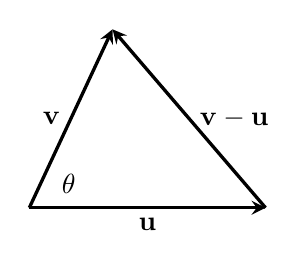
\begin{tikzpicture}[vector/.style={-stealth,very thick}]
            \coordinate (O) at (0,0);
            \coordinate (A) at (3,0);
            \coordinate (B) at (65:2.5);

            \draw[vector] (O) -- (A) node[midway,below] {$\mathbf{u}$};
            \draw[vector] (O) -- (B) node[midway,left] {$\mathbf{v}$};
            \draw[vector] (A) -- (B) node[midway,right] {$\mathbf{v-u}$};
            \node at (0.5,0.3) {$\theta$};
        \end{tikzpicture}
    \]

    \subsubsection{Exercise} Use the Cosine rule to show that
    \[ \mathbf{u} \cdot \mathbf{v} = |\mathbf{u}| | \mathbf{v}| \cos{\theta}. \]

    \subsection{Finding the angle between two vectors} The result from the exercise above can be restated in terms of $\cos{\theta}$:
    \[ \cos{\theta} = \frac{\mathbf{u} \cdot \mathbf{v}}{|\mathbf{u}||\mathbf{v}|.} \]
    Taking the arccosine of both sides then gives us a value for $\theta \in [0, \pi]$. This value is taken to be the angle between two vectors.

    \subsubsection{Exercise} Show that two vectors $\mathbf{u}, \mathbf{v} \in \mathbb{R}^n$ are \textbf{orthogonal} (at $90^\circ$ or $\frac{\pi}{2}$ radians)  if and only if $\mathbf{u} \cdot \mathbf{v} = 0$.

\end{document}